\subsection{Feldorientierte Regelung (FOC)}\label{Feldorientierte Regelung}
	Mithilfe der feldorientiereten Regelung ist es m�glich das Feld des Stators so anzupassen, dass es dem Feld des Rotors genau so vorl�uft, dass Drehmoment und Effizienz maximiert werden. Im Gegensatz zur BLDC-Regelung kann das Statorfeld nicht nur 6 Positionen annehmen, sondern unbegrenzt viele. Man kann mit dieser Methode auch eine etwas h�here Drehzahl erreichen. Um diese 90� Verschiebung des Statorfelds zu erreichen, wird der Feldvektor zun�chst in seine zwei Komponenten Id und Iq, welche 90Grad zueinander liegen, aufgeteilt:
	
	\begin{figure}[H]
			\centering
			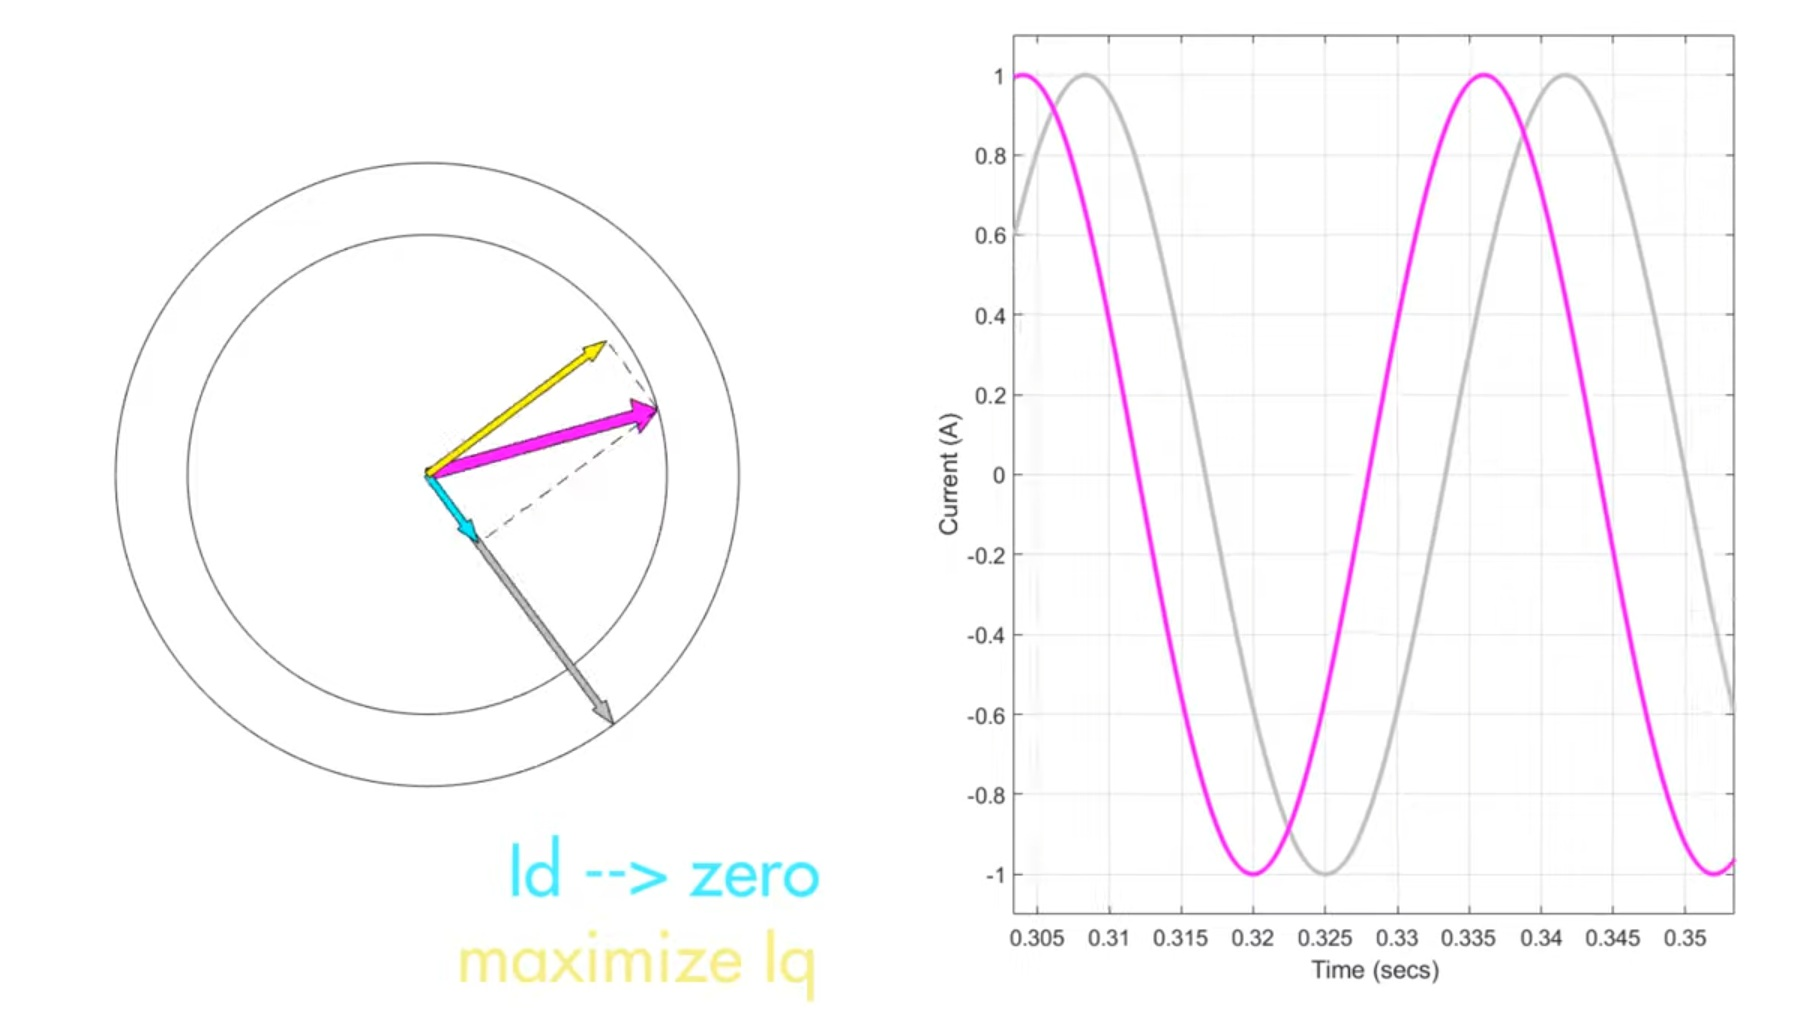
\includegraphics[scale=0.25]{./3_Stand_der_Technik/Abbildungen/FOC_Control_1}
			\caption{Komponenten des Statormagnetfelds\cite{MATLAB2020}}
	\end{figure}
	
	Das Ziel des Reglers ist demnach Id gegen 0 zu regeln und Iq entsprechend dem gew�nschten Drehmoment so hoch wie m�glich zu regeln.
	
	Der Aufbau eines FOC-Algorhitmus ist in der Regel wiefolgt:
	
	\begin{figure}[H]
			\centering
			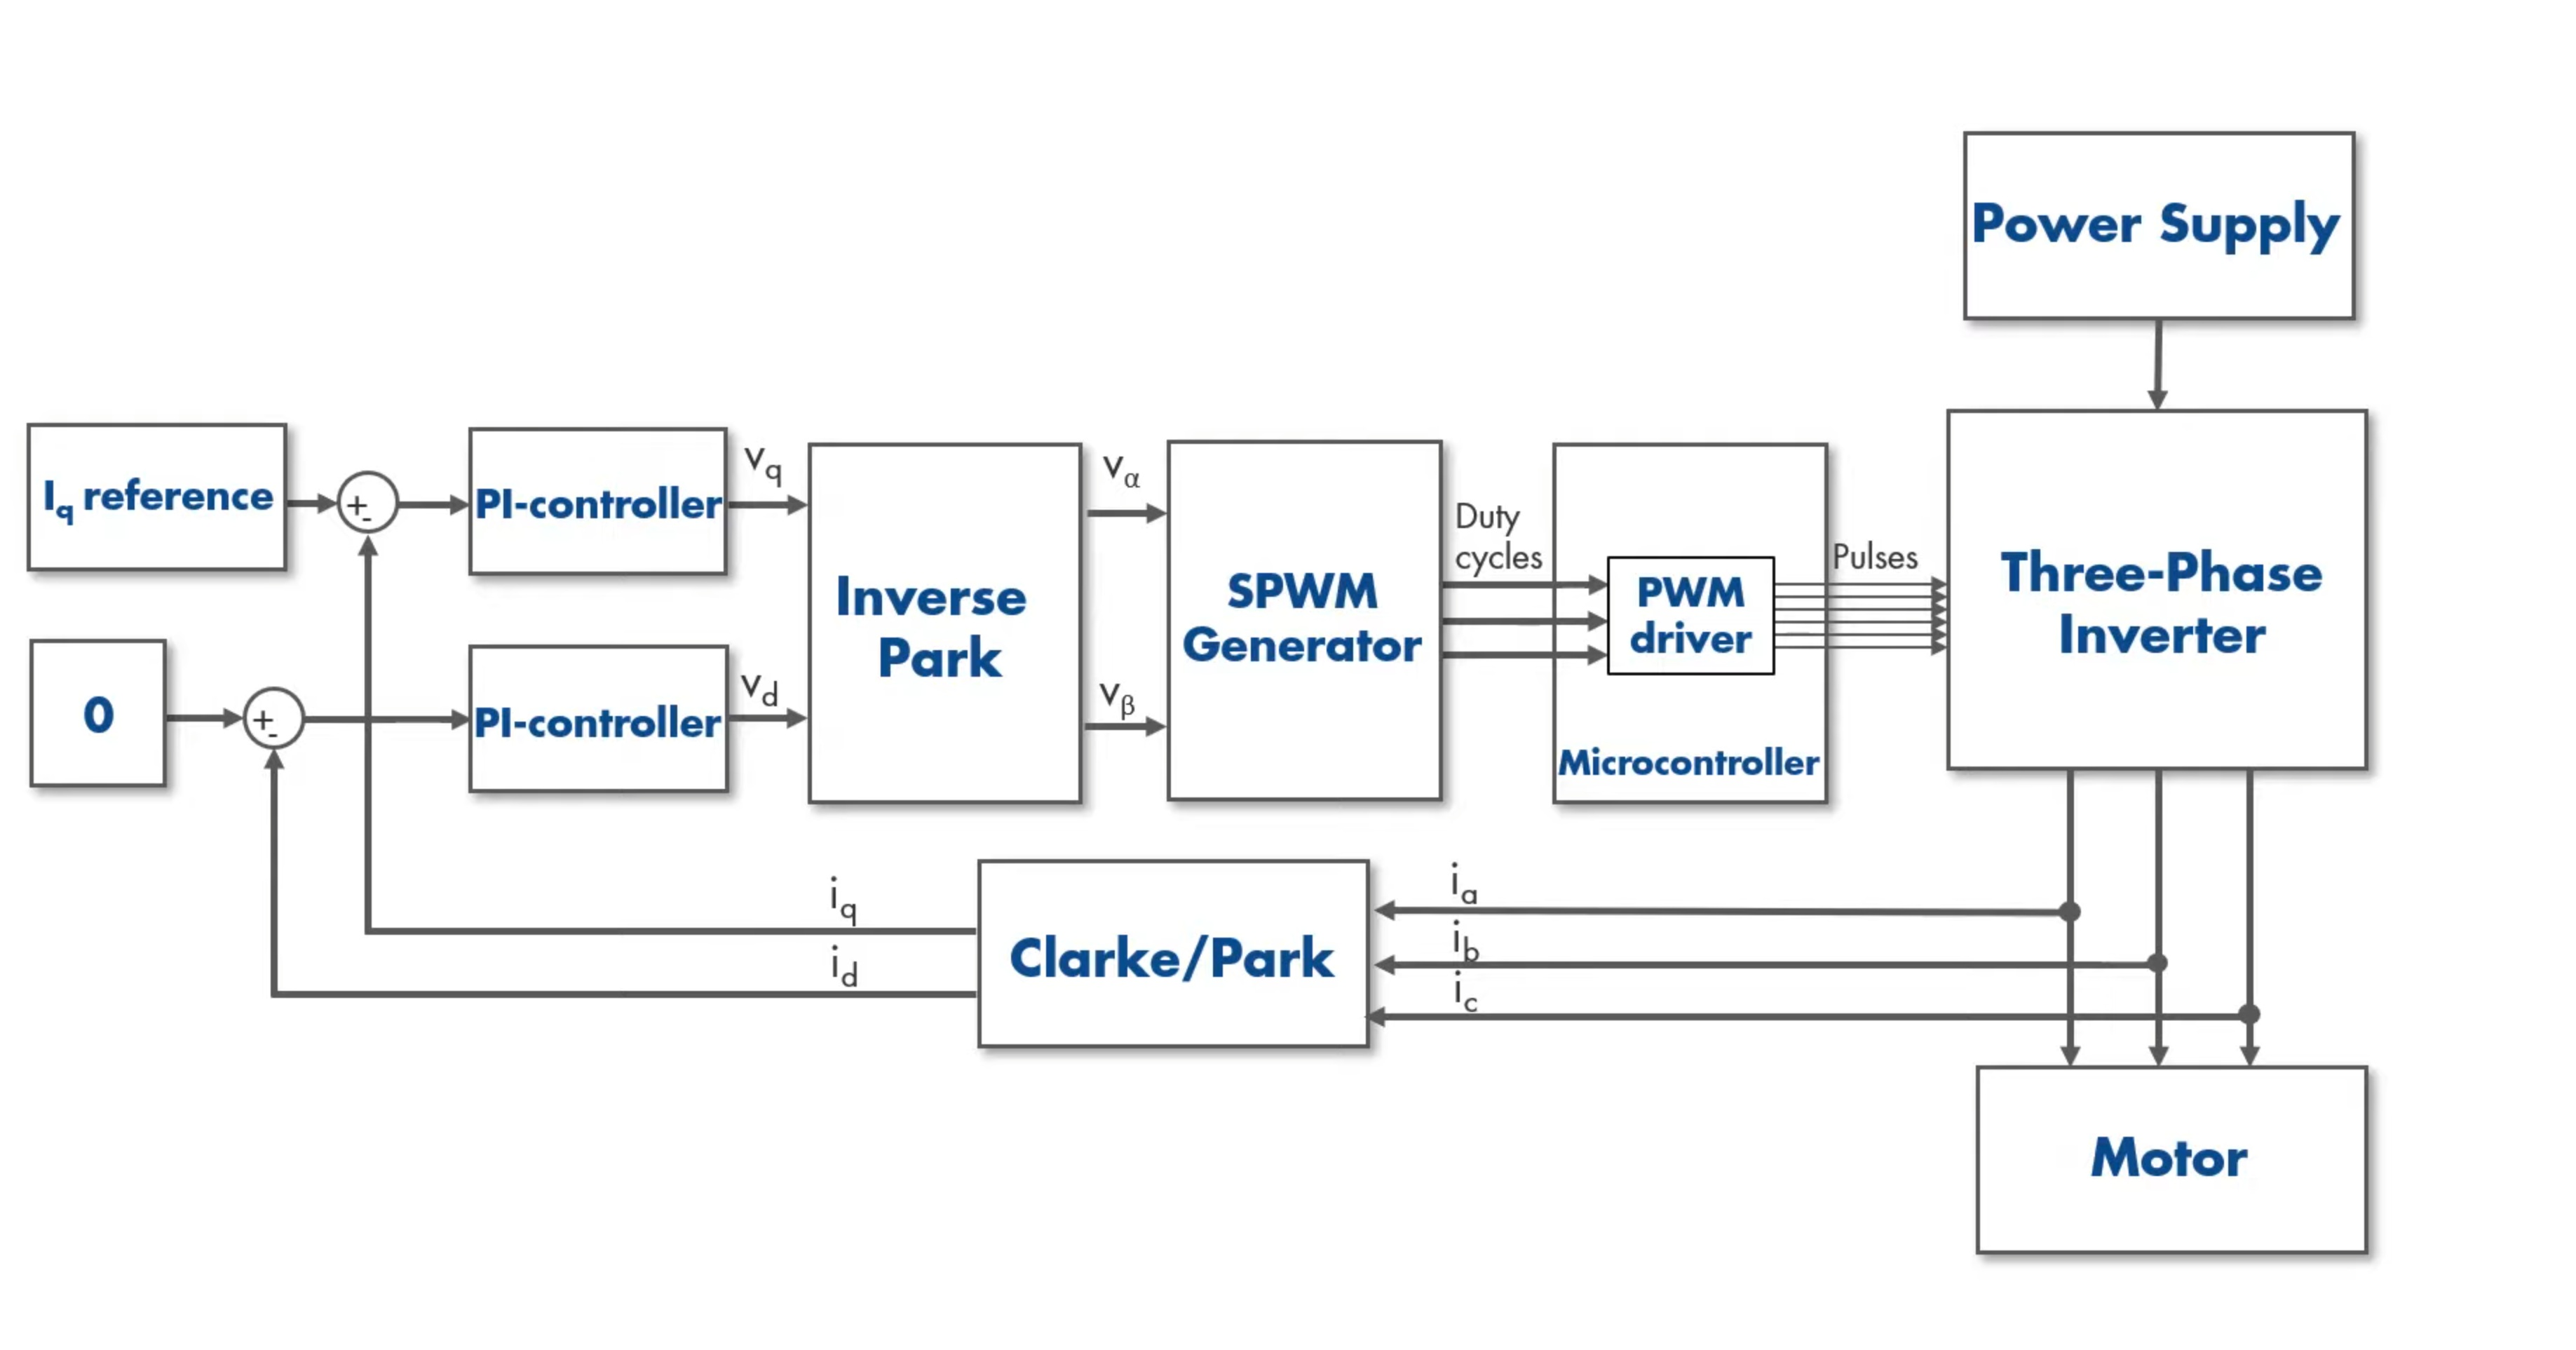
\includegraphics[scale=0.2]{./3_Stand_der_Technik/Abbildungen/FOC_Control_2}
			\caption{Aufbau eines FOC-Algorhitmus\cite{MATLAB2021}}
	\end{figure}
	
	Mithilfe von Shunts wird der derzeitige Statorstrom zum Motor gemessen. Diese Werte werden mithilfe von mathematischen Transformationen (Clark- und Park Transformation) in die zwei Anteile Id und Iq umgerechnet, welche zusammen den Strom des Statorfelds ergeben. Auch wird mithilfe eines Positionssensors die Position des Rotors gemessen.
	Zwei PI-Regler regeln nun Id auf 0 und Iq auf den gew�nschten Eingangsstrom. Anschlie�end werden die Werte mithilfe von mathematischen Transformationen(inverse Clark Transformation) in die Spannungswerte Vd und Vq umgerechnet. Diese Spannungen entsprechen jedoch noch nicht den gew�nschten Strangspannungen des Motors, sondern m�ssen mithilfe von Ortsvektor-Modulierung in pulsweitenmodulierte Signale f�r den Wechselrichter umgerechnet werden:
	
	Der Ortsvektor des Stators beschreibt die Position des Statormagnetfelds. Es ergibt sich durch Addieren der 3 Strangstr�me.
	
	\begin{figure}[H]
			\centering
			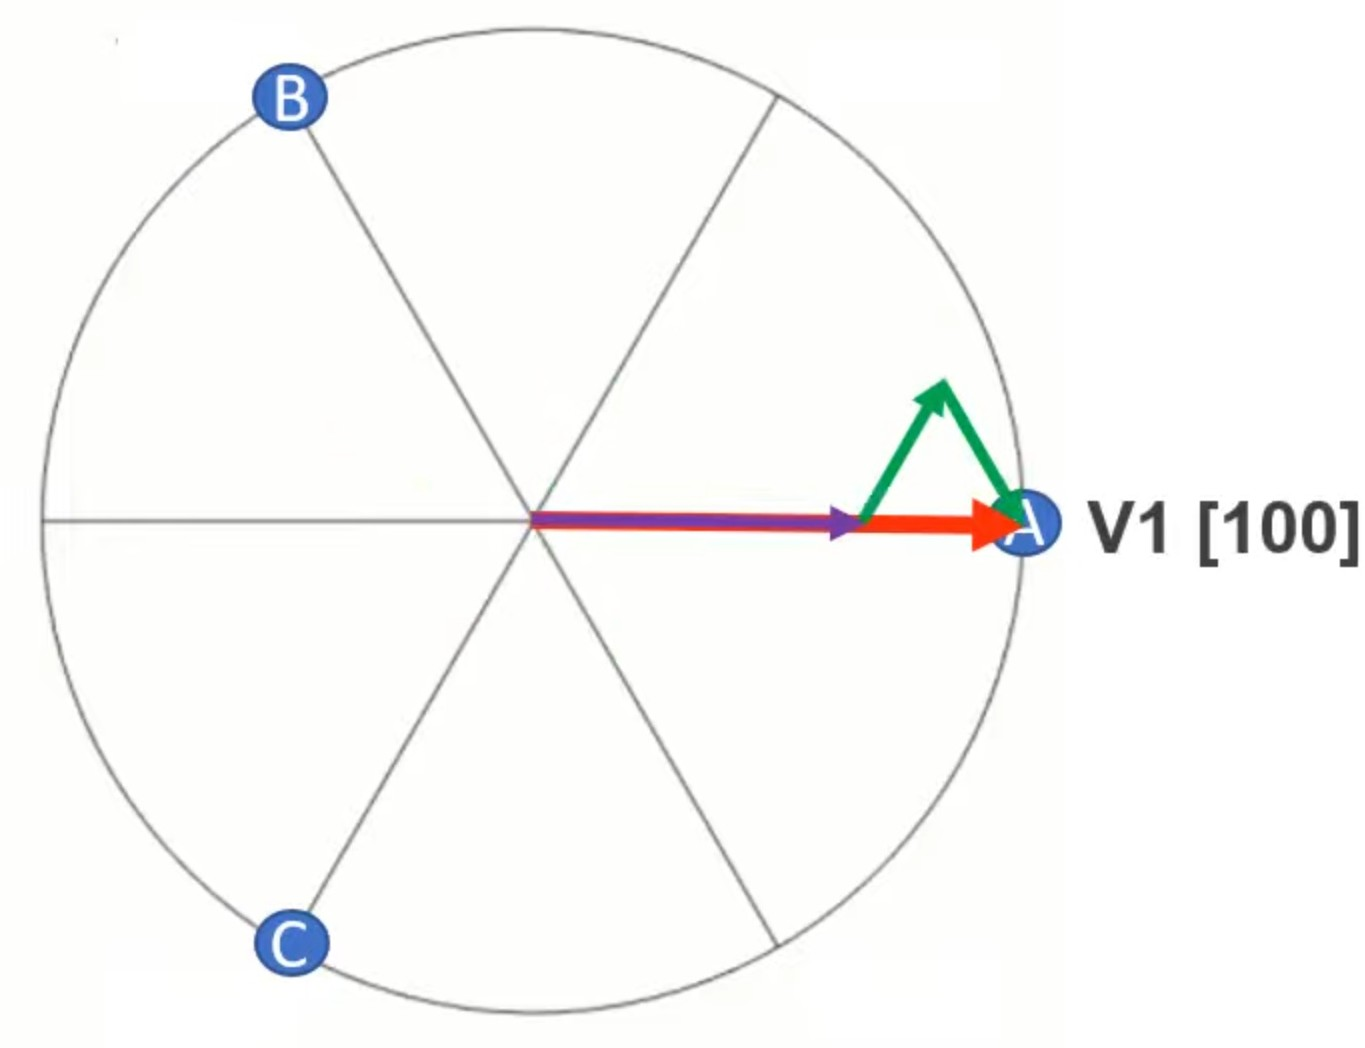
\includegraphics[scale=0.3]{./3_Stand_der_Technik/Abbildungen/FOC_Control_3}
			\caption{Ortsvektor\cite{MATLAB2021}}
	\end{figure}
	
	Der Wechselrichter kann grunds�tzlich 8 unterschiedliche Schaltpositionen annehmen. Bei zwei von diesen flie�t kein Strom. Die anderen entsprechen folgenden 6 Rotorposiotionen

	\begin{figure}[H]
			\centering
			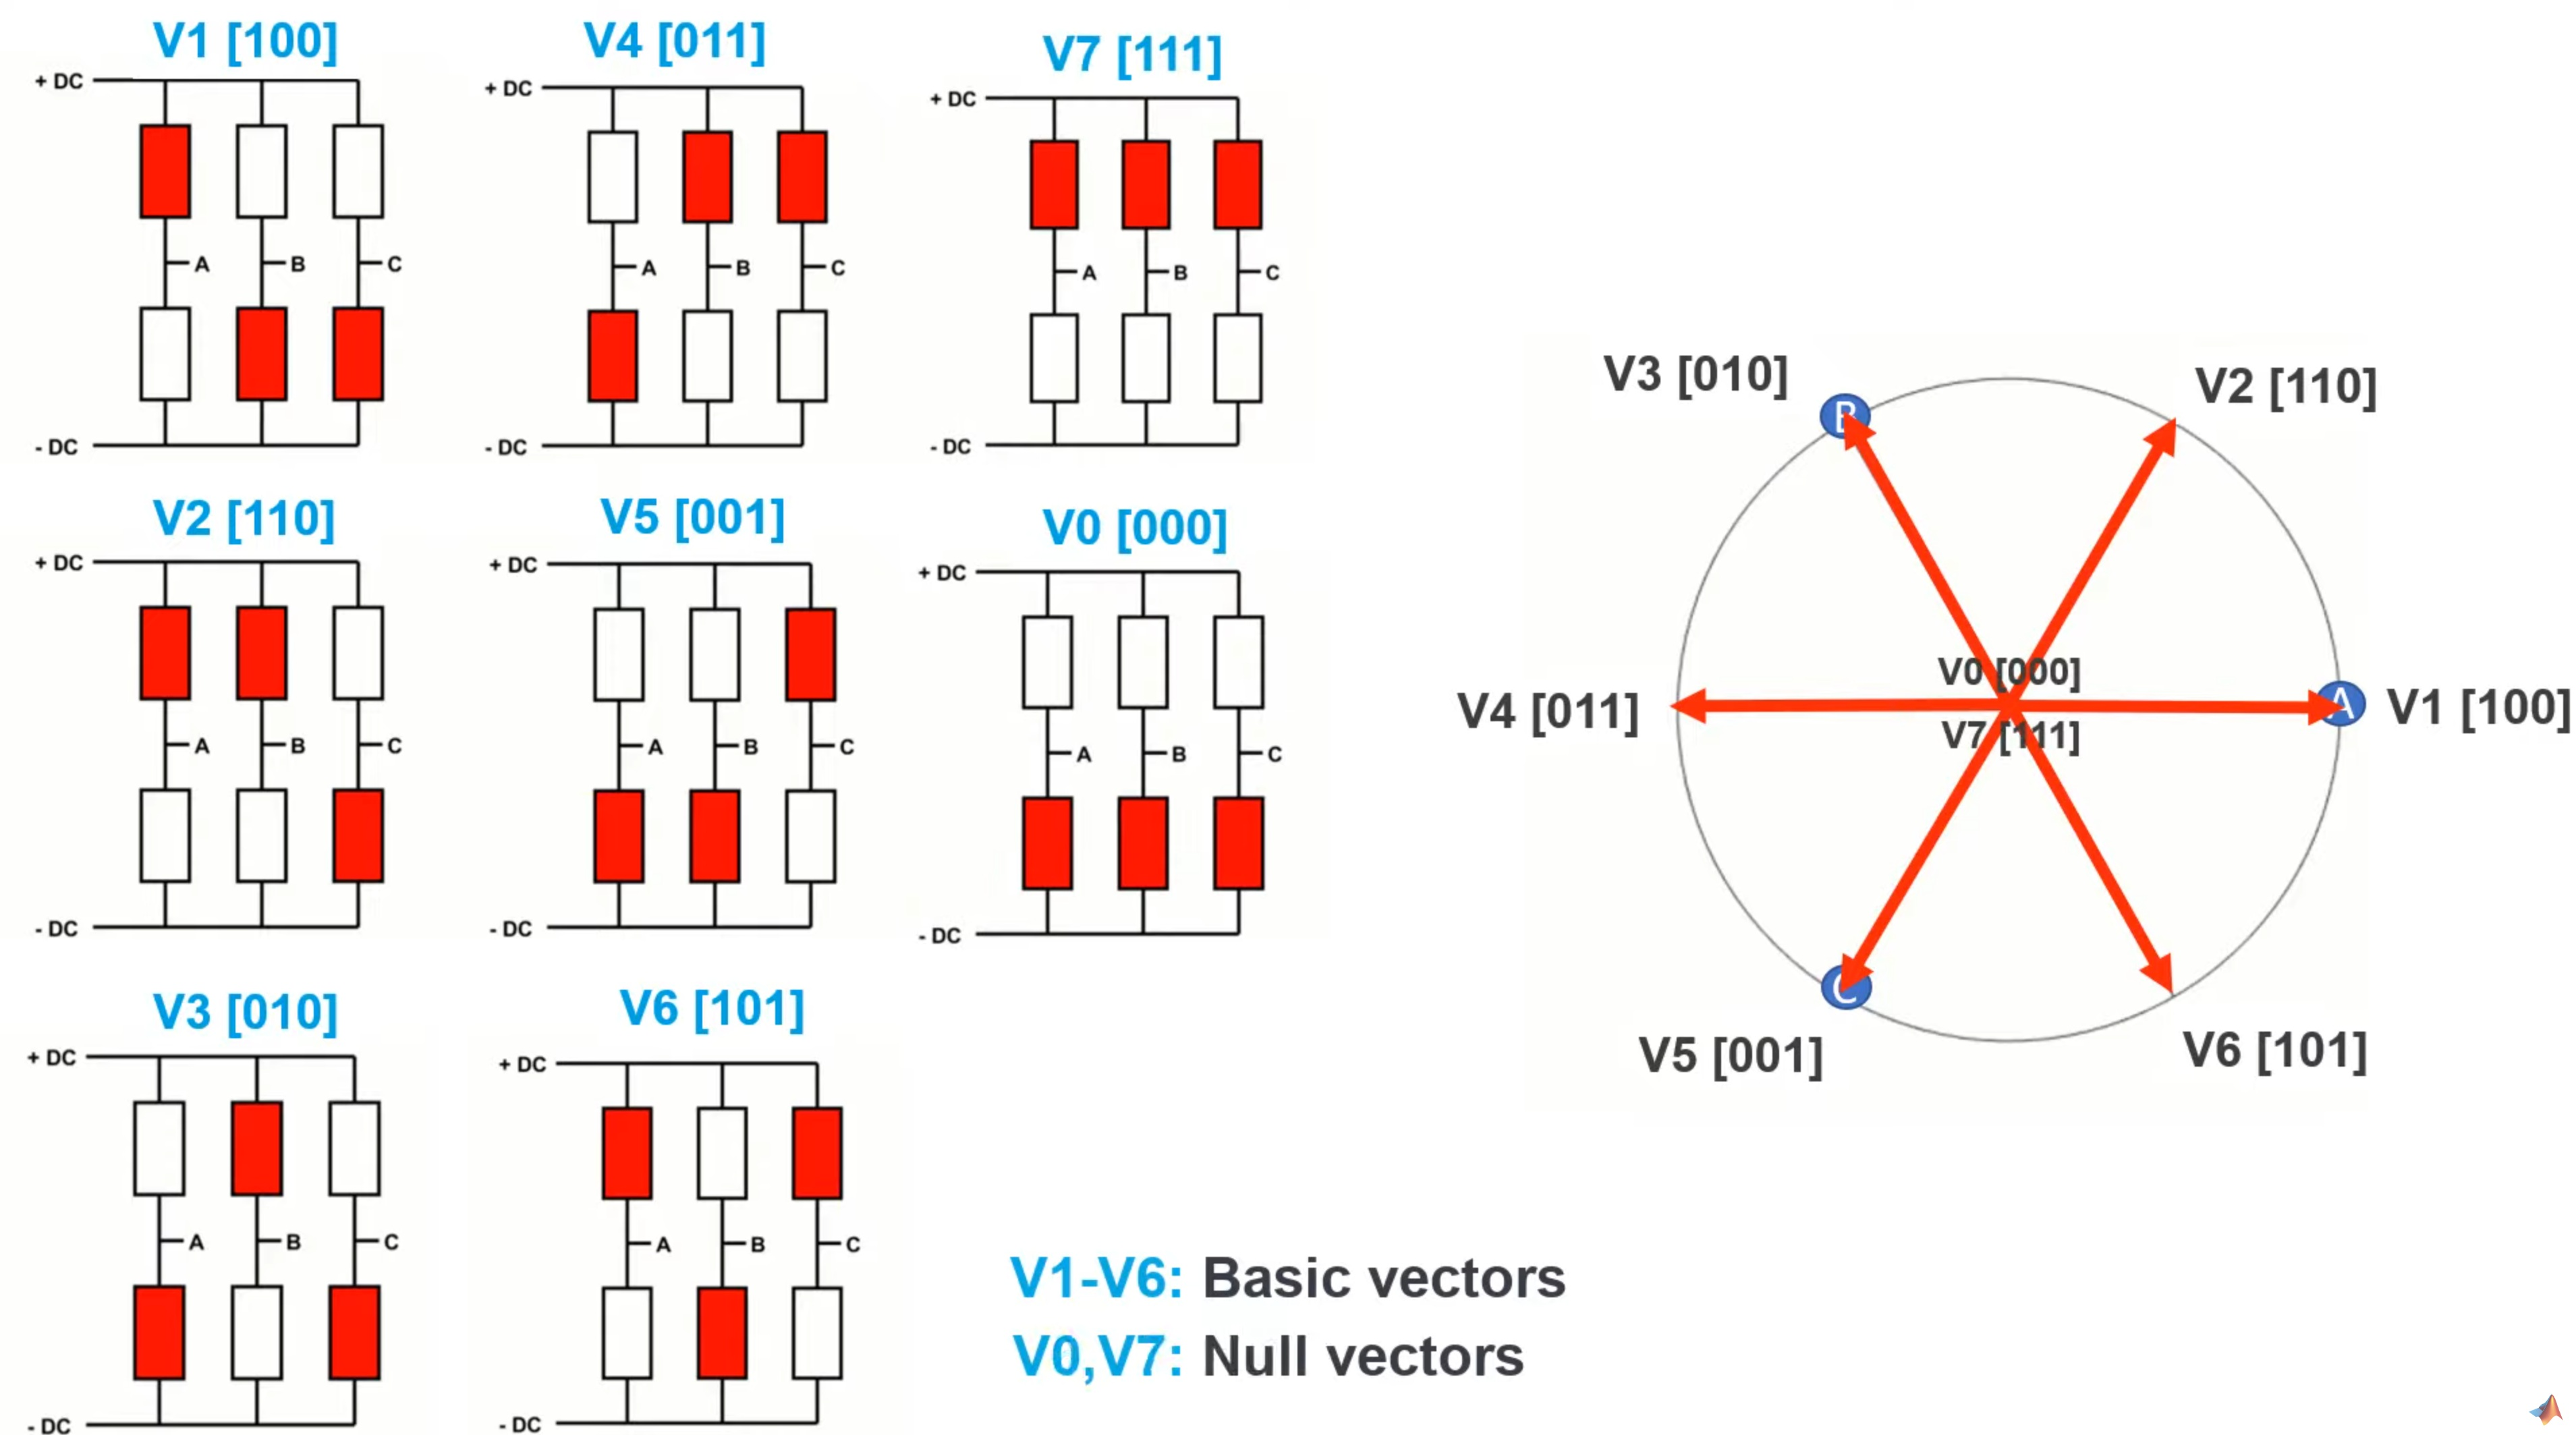
\includegraphics[scale=0.2]{./3_Stand_der_Technik/Abbildungen/FOC_Control_4}
			\caption{Ortsvektoren des Wechselrichters\cite{MATLAB2021}}
	\end{figure}
	
	Indem mit hoher Frequenz geziehlt zwischen diesen Ortsvektoren geschalten wird(pulsweitenmodulierte Signale) kann ein resultierender Ortsvektor an jeder Position des Kreises entstehen. So kann Drehmoment und Drehzahl ohne Schwankungen genau geregelt werden.\cite{MATLAB2021}
